\textbf{An introduction to the \textbf{patterns} associated with peer
learning.} Consider the following learning scenarios:

\begin{enumerate}
\item
  A study group for a tough class in Honors Physics convenes at at the
  library late one night, resolving to do well on the next day's exam.
  The students manage to deflect their purpose for a while by gossiping
  about hook-ups and parties, studying for other classes, and sharing
  photos. Then, first one member, then another, takes the initiative and
  as a group, the students eventually pull their attention back to the
  task at hand. They endure the monotony of studying for several hours,
  and the next day, they own the exam.
\item
  A young skateboarder spends hours tweaking the mechanics of how to
  make a skateboard float in the air for a split second, enduring
  physical pain of repeated wipeouts. With repetition and success comes
  a deep understanding of the physics of the trick. That same student
  cannot string together more than five minutes of continuous attention
  during class and spends even less time on homework for the class
  before giving up.
\end{enumerate}
Peer-learning participants succeed when they are motivated to learn.
Skateboarding is primarily intrinsically motivated, with some extrinsic
motivation coming from the respect that kids receive from peers when
they master a trick. In most cases, the primary motivation for learning
physics is extrinsic, coming from parents' and society's expectations
that the student excel and assure his or her future by getting into a
top college.

The student very well could be intrinsically motivated to have a glowing
report card, but not for the joy of learning physics, but because of the
motivation to earn a high grade as part of her overall portfolio. Taken
a different way, what is it about physics that's fun for a student who
does love the science? Perhaps she anticipates the respect, power and
prestige that comes from announcing a new breakthrough; or she may feel
her work is important for the greater good, or prosperity, of humanity;
or she may simply be thrilled to see atoms bonding to form new
compounds.

Learning situations frequently bore the learner when extrinsic
motivation is involved. Whether by parents or society, being forced to
do something, as opposed to choosing to, ends up making the individual
less likely to succeed. In some cases it's clear, but trying to figure
out what makes learning fun for a group of individual humans can be very
difficult. Often there is no clear-cut answer that can be directly
applied in the learning environment. Either way, identifying the factors
that can make learning boring or fun is a good start. Perhaps learning
certain skills or topics is intrinsically boring, no matter what, and we
have to accept that.

\begin{figure}
\begin{center}
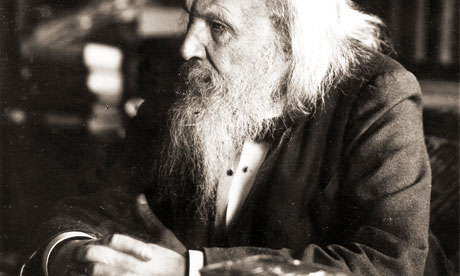
\includegraphics[width=.8\textwidth]{../pictures/mendeleev.jpg}
\end{center}
\caption*{Photo of Dmitri Mendeleev (1834-1907). Found on The Guardian's Notes \&
Theories blog. Public domain.}
\end{figure}

\subsubsection{Learning patterns}

One way to think about fun learning is that it's fun to learn - and be
aware that you're learning - new patterns. Jürgen Schmidhuber wrote: ``A
{[}\ldots{}{]} learner maximizes expected fun by finding or creating
data that is better compressible in some yet unknown but learnable way,
such as jokes, songs, paintings, or scientific observations obeying
novel, unpublished laws'' {[}1{]}. So the skateboarder enjoyed coming
across new patterns: novel tricks that were nonetheless learnable.

\subsection{Learner, know thyself: a self-evaluation technique}

The learning contributed and acquired by each member of the peer
learning enterprise depends on a healthy sense of self-awareness. When
you ask yourself, ``What do I have to offer?'' and ``What do I get out
of it?'' we think you'll come up with some exciting answers. In peer
learning, whether or not you're pursuing a practical objective, you're
in charge, and this kind of learning is usually fun. Indeed, as we'll
describe below, there are deep links between play and learning. We
believe we can improve the co-learning experience by adopting a playful
mindset. Certainly some of our best learning moments in the Peeragogy
project have been peppered with humor and banter. So we found that a key
strategy for successful peer learning is to engage in a self-assessment
of your motivations and abilities. In this exercise, you take into
account factors like the learning context, timing and sequence of
learning activities, social reinforcements, and visible reward. The
peeragogical view is that learning is most effective when it contains
some form of enjoyment or satisfaction, or when it leads to a concrete
accomplishment.

When joining the Peeragogy project, Charles Jeffrey Danoff did a brief
self-evaluation about what makes him interested in learning:

\begin{enumerate}
\item
  \textbf{Context}. I resist being groomed for some unforeseeable future
  rather than for a specific purpose.
\item
  \textbf{Timing and sequence}. I find learning fun when I'm studying
  something as a way to procrastinate on another pressing assignment.
\item
  \textbf{Social reinforcement}. Getting tips from peers on how to
  navigate a snowboard around moguls was more fun for me than my Dad
  showing me the proper way to buff the car's leather seats on chore
  day.
\item
  \textbf{Experiential awareness}. In high school, it was not fun to sit
  and compose a 30-page reading journal for Frankenstein. But owing in
  part to those types of prior experiences, I now find writing
  pleasurable and it's fun to learn how to write better.
\end{enumerate}
We will explore the patterns of peer learning in more detail in the
section on \href{http://peeragogy.org/practice/}{practice}.

\subsection{Reference}

\begin{enumerate}
\item
  Schmidhuber, J. (2010). Formal theory of creativity, fun, and
  intrinsic motivation. Autonomous Mental Development (IEEE), 2(3),
  230-247.
\end{enumerate}
